\clearpage % guidance only
\section{Bias}
As explained in \autoref{sec:dsea:dsea},
\dsea{} is intended to eliminate the bias introduced by the energy spectrum of the Monte Carlo training data.
%
In order to test
whether the bias is indeed eliminated,
the model is evaluated on a \emph{stratified} dataset,
    where each bin contains an equal number of events,
whereas the training data is the same as before.
% TODO: explain that dataset(s): number of events etc.
\todo{
  Samuel did the opposite: stratified training data, but not test data.
  I should consider doing the same. (@Leonora)
}

The results are shown in \autoref{fig:bias_comparison}.
As can be seen,
The model adapts to the unseen distribution of the test data.
No bias is observed.

… in comparison to \autoref{fig:bootstrap:spectrum}.

% TODO: Move to summary?
In comparison,
in the work by \citeauthor{dsea_samuel},
relative deviations of more than \SI{1500}{\percent} are observed \cite{dsea_samuel}.
% Aber er schiebt's auf die geringe Accuracy…


\begin{figure}
  \centering
  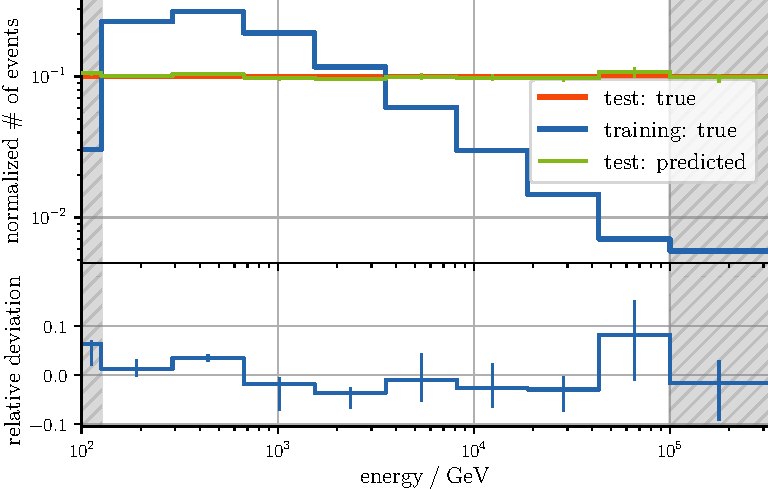
\includegraphics[scale=1]{content/plots/bias:spectrum_full.pdf}
  \caption{
    Energy spectrum and relative deviations…
    % TODO gleichverteilte Klassen… bla…
  }
  \label{fig:bias_comparison}
\end{figure}
